\documentclass{article}
\usepackage[toc]{glossaries}
\usepackage[utf8]{inputenc}
\usepackage{supertabular}
\usepackage[T1]{fontenc}
\usepackage{icomma}
\usepackage{array} 
\usepackage{color}
\usepackage{amsmath,mathtools}
\usepackage{amssymb,amsfonts}
\usepackage{esint}
\usepackage{multirow}
\usepackage{float}
\usepackage{graphicx}
\usepackage{tikz}
\usepackage[left=2.5cm,right=2.5cm,top=3cm,bottom=3cm]{geometry}
\usepackage{hyperref}
\usepackage[portuguese]{babel}
\usepackage{caption}
\usepackage[bottom]{footmisc}
\usepackage{gensymb}
\usepackage{tabulary}
\usepackage{fancyhdr}
\usepackage{siunitx}
\usepackage{textcomp}
\usepackage[siunitx]{circuitikz}
\newcommand{\HRule}{\rule{\linewidth}{0.5mm}}
\usepackage{parskip}
\setlength{\parindent}{20pt}
\setlength{\parskip}{15pt}
\setlength\extrarowheight{2pt}
\usepackage{tcolorbox}
\usepackage{enumitem}
\usepackage[ampersand]{easylist}
\usepackage{subfigure}
\usepackage{hhline}
\usepackage{datetime}
\usepackage{fancyhdr}
\pagestyle{fancy}
\usepackage{lastpage}
\renewcommand\headrulewidth{1pt}
\usepackage{biblatex} 
\addbibresource{Bibliography.bib} 
\usepackage{csquotes}
\usepackage{calligra}
\usepackage{physics}

\DeclareFontShape{T1}{calligra}{m}{n}{<->s*[2.2]callig15}{}
\newcommand{\scripty}[1]{\ensuremath{\mathcalligra{#1}}}


\fancyhead[L]{\textbf{Sistemas Baseados em Similaridade}}
\fancyhead[C]{}
\fancyhead[R]{Universidade do Minho}
\renewcommand\footrulewidth{1pt}
\fancyfoot[C]{\textbf{Page \thepage/\pageref{LastPage}}}
\fancyfoot[R]{\today}
\makeindex
\makenoidxglossaries
\newglossaryentry{heralds}
{
    name=Herald,
    description={Exemplos de um \textit{elite monster}}
}

\newglossaryentry{wards}
{
    name=Wards,
    description={Unidades plantáveis que removem a névoa da guerra numa determinada área do mapa}
}

\newglossaryentry{firstBlood}
{
    name=First Blood,
    description={Consequência de ser o primeiro campeão em ambas a equipas e obter uma \textit{kill}. Concede um bónus de \textit{gold} ao campeão em causa e ao campeão que condece a respetiva \textit{assist}}
}

\newglossaryentry{kills}
{
    name=Kills,
    description={Ações de matar um campeão adversário}
}

\newglossaryentry{assists}
{
    name=Assists,
    description={Ações de ajudar um campeão aliado a matar um campeão adversário}
}

\newglossaryentry{eliteMonster}
{
    name=Elite Monsters,
    description={Unidades neutras, fortes e difíceis de matar, que concedem \textit{buffs} a toda a equipa e/ou altas recompensas de \textit{gold}/experiência}
}

\newglossaryentry{dragons}
{
    name=Dragons,
    description={Exemplos de um \textit{elite monster}}
}

\newglossaryentry{torres}
{
    name=Torres,
    description={Estruturas que atacam campeões adversários, e que devem ser destruídas para avançar no jogo}
}

\newglossaryentry{gold}
{
    name=Gold,
    description={Unidade monetária que permite a compra de itens na loja}
}

\newglossaryentry{experiencia}
{
    name=Experiência,
    description={Mecânica do jogo que permite um campeão subir de nível}
}

\newglossaryentry{minions}
{
    name=Minions,
    description={Unidades geradas periodicamente que atacam campeões/estruturas adversárias}
}

\newglossaryentry{jungleMinions}
{
    name=Jungle Minions,
    description={Unidades neutras encontradas na \textit{Jungle} que concedem \textit{gold} e experiência}
}

\newglossaryentry{nivel}
{
    name=Nível,
    description={Mecânica do jogo que determina se um campeão pode aceder a determinadas \textit{features}}
}



\begin{document}
\begin{titlepage}
\begin{center}

\includegraphics[scale=0.6]{uminho.png}
\line(1,0){400}\\
[2mm]
\begin{large}
\textbf{Trabalho Prático de Grupo Nº1}\\ 
\end{large}
\line(1,0){250}\\
[1.5cm]
Realizado por:\\ 
\vspace{5mm}
Benjamim Oliveira PG42815\\
Gonçalo Almeida A84610\\
Nuno Pereira PG42846\\
Rui Reis A84930\\
[4cm]
No âmbito do cursos:\\
MEIE/MEI/MMC\\ 
[2.5cm]
Unidade Curricular:\\
SBS (Sistemas Baseados em Similaridade)
\end{center} 
\end{titlepage}
\tableofcontents
\newpage
 
% ---------------------------------------------------------------------------
% 1) INTRODUCAO E CONTEXTUALIZACAO
\section{Introdução \& Contextualização}

Este trabalho foi desenvolvido no âmbito na unidade curricular "Sistemas Baseados em Similaridade", do perfil "Machine Learning: Fundamentos e Aplicações", do conjunto de cursos MIEI/MEI/MMC, disponibilizados pela Universidade do Minho.

De forma paralela foram explorados dois \textit{datasets}, um fornecido pelos docentes da unidade curricular e o outro escolhido por nós. O \textit{dataset} fornecido visa registos de incidentes rodoviários na cidade de Braga ao longo do ano de 2019, contendo dados como a magnitude do atraso gerado pelos incidentes, as estradas afectadas, o atraso em segundos provocado pelo acidente, entre muitos outros. O nosso objetivo é prever qual a magnitude de incidentes de cada registo com a maior precisão possível, este parâmetro pode assumir 5 valores distintos dentro do conjunto $C_1 = \{\mbox{\texttt{None}, \texttt{Low}, \texttt{Medium}, \texttt{High}, \texttt{Very\_High}}\}$.

O segundo \textit{dataset} utilizado incide sobre partidas do videojogo de \textit{League of Legends}, mais concretamente, sobre os primeiros 10 minutos das mesmas. \textit{League of Legends} é um jogo multi-player online, em que duas equipas de 5 jogadores se defrontam numa partida com uma duração média de 30 a 40 minutos. Com este estudo pretendemos perceber o quão forte é o efeito dos primeiros 10 minutos numa partida em garantir a vitória. 

%\section{Domínios a tratar}
\subsection{Objetivos}
Este trabalho foi desenvolvido no âmbito na unidade curricular "Sistemas Baseados em Similaridade", do perfil "Machine Learning: Fundamentos e Aplicações", do Mestrado em Engenharia Informática, disponibilizado pela Universidade do Minho.

De forma paralela foram explorados dois \textit{datasets}, um fornecido pelos docentes da unidade curricular e um por nós escolhido. O \textit{dataset} fornecido visa registos de incidentes rodoviários na cidade de Braga, contendo dados como a magnitude do atraso gerado pelos incidentes, as estradas afetadas ou o atraso em segundos provocado pelo acidente. O nosso objetivo concreto é prevermos qual o nível de incidentes de cada registo com a maior precisão possível, este parâmetro pode ter 5 valores diferentes, entre "None" e "Very High".

O segundo \textit{dataset} utilizado incide sobre partidas de League of Legends, mais concretamente sobre os primeiros 10 minutos da mesma. League of Legends é um jogo multi-player online, em que duas equipas de 5 jogadores se defrontam. No mapa onde a partida acontece existem diversos objetivos espalhados que dão vantagens á equipa que os conquistar. O objetivo a que nos propomos consiste em tentar prever qual será a equipa vencedora, baseando esta previsão nos primeiros 10 minutos de jogo.

\subsection{Proposta de resolução}
Para atingir ambos os objetivos propomos-nos a desenvolver modelos de machine learning, através de \textit{Random Forest}, fazendo uso de conhecimentos adquiridos em aula. Para desenvolver estes modelos é utilizado Knime, sendo desenvolvidos diferentes processos para preparar os dados, optimizar os parâmetros do modelo e optimizar o mesmo.

% ---------------------------------------------------------------------------
% 2) METODOLOGIA CRISP-DM
\section{Metodologia CRISP-DM}

De forma a garantir a qualidade dos modelos produzidos ao longo deste estudo, a metodologia \textit{Cross Industry Standard Process for Data Mining}, ou CRISP-DM, foi empreendida no intuito de garantir inclusão de abordagens normalmente utilizadas pelos profissionais da área com vantagens imediatas na qualidade do projecto desenvolvido.

\begin{figure}[H]
    \centering
    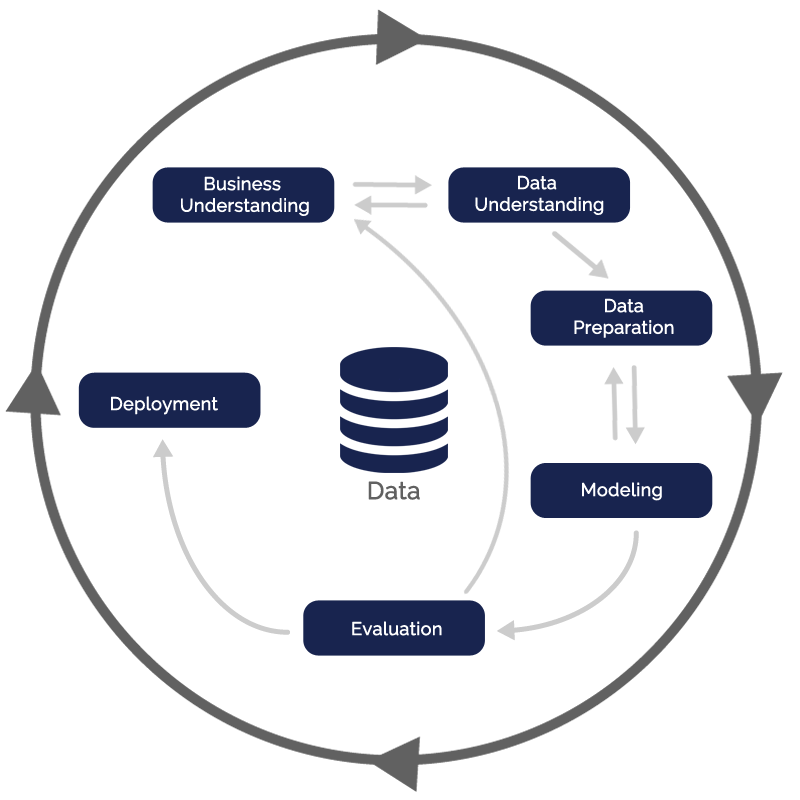
\includegraphics[width=0.4\linewidth]{Figures/crispdm.png}
    \caption{Diagrama ilustrativo da metodologia CRISP-DM.}
    \label{fig:s2i1}
\end{figure}

A figura \ref{fig:s2i1} ilustra os passos considerados por esta metodologia. De imediato, é possível perceber que esta metodologia não possui um início ou fim bem definido, propositadamente este comportamento é definido de forma a conseguir garantir que existe um refinamento do projecto ao longo do tempo, cada iteração contemplando das informações colectadas pela iteração anterior. Esta metodologia pode ser, resumidamente, descrita nos seguintes termos.

\begin{enumerate}
    \item \textbf{Compreensão do Negócio} - É importante perceber qual é o domínio do negócio/tema que estamos a considerar, o que estamos a tentar prever e como utilizar o nosso conhecimento de domínio em nosso prol.
    \item \textbf{Compreensão dos Dados} - Compreender o conjunto de dados captados, como os utilizar para alcançar o nosso objetivo e explorar estes de forma a descobrir fatores de interesse.
    \item \textbf{Preparação dos Dados} - Perceber qual a melhor forma para processar os dados de tal forma a que os modelos desenvolvidos possam tirar mais proveito.
    \item \textbf{Modelação} - Pesar os diferentes modelos utilizados, a diferenças entre si para alcançar o objetivo, bem como ponderar a variação dos hyper-parâmetros.
    \item \textbf{Apreciação} - Comparar o modelo com os objetivos iniciais propostos e perceber de que forma o modelo permite descrever o desejado.
\end{enumerate}

É importante ter em conta que a fase denotada como \textit{Deployment} da figura \ref{fig:s2i1} foi propositadamente deixada de parte, por não ter sido considerada em grande amplitude ao longo deste projeto.

% ---------------------------------------------------------------------------
% 3) ACIDENTES BRAGA
\section{Acidentes em Braga no ano de 2019}

% todo este conteudo, ate a proxima subsection, corresponde, na pratica,
% à componente de Business Understanding do CRISP-DM
Segundo a PORDATA\footnote{\url{https://www.pordata.pt/Portugal/Acidentes+de+via\%c3\%a7\%c3\%a3o+com+v\%c3\%adtimas++feridos+e+mortos+++Continente-326}}, no ano de 2018, em Portugal, foram registados $34235$ acidentes rodoviários com vítimas, totalizando $508$ vítimas mortais. Como tal, a motivação para o desenvolvimento de um trabalho deste tipo é imediata.

Ao conseguirmos compreender melhor os factores que causam acidentes, trabalhando em específico com os dados da zona de Braga, pretendemos ser capazes de generalizar e compreender quais atributos são os mais informativos no sentido de prever o número de acidentes num determinado dia.

Com um modelo capaz de efectivamente utilizarmos os atributos mais informativos, na prática seriamos capazes de desenvolver campanhas personalizadas para promover a segurança rodoviária, entre outras medidas cujo impacto possa ser directamente mensurável a partir do nosso modelo.

% STEP 2 IN CRISP DM METODOLY
\subsection{Compreensão dos Dados}
Os dados utilizados neste ponto foram cedidos pelos docentes da unidade curricular e versam incidentes rodoviários na cidade de Braga no ano de 2019.

Estes dados focam informações como por exemplo:
\begin{itemize}
    \item As estradas afetadas num determinado momento
    \item O atraso causado pelo incidente
    \item O dia e hora do incidente
\end{itemize}

No conjunto de dados inicial temos 13 colunas.



% STEP 3 IN CRISP DM METODOLOGY
\subsection{Preparação dos Dados}
A nível de preparação de dados pouco foi feito, no entanto é importante denotar os seguintes aspectos chaves, que foram cruciais na nossa investigação.

\begin{itemize}
    \item A atributo \texttt{gameID} é completamente irrelevante pois é uma chave única associada a cada jogo, sem nenhum tipo de relevància física, por isso esse atributo foi removido.
    \item Os atributos \texttt{blueWins} e \texttt{redWins} são ambos binários e disjuntos, o que significa que a soma será sempre 1, pois numa dada partida apenas uma equipa pode ganhar. Como tal, consideramos apenas o atributo \texttt{blueWins}, tornando o problema num de prever a vitória ou derrota desta mesma equipa.
    \item De igual forma, os atributos \texttt{blueFirstBlood} e \texttt{redFirstBlood} seguem a mesma condição, pelo que só vale a pena ponderar um destes atributos.
    \item Nos restantes atributos, considerar tanto os atributos da equipa azul e vermelha não faz sentido. Na verdade, estamos interessados em perceber qual a diferença entre os resultados obtidos pela equipa azul num dado atributo e aqueles obtidos pela equipa vermelha. Assim sendo, os restantes atributos, 36, foram reduzidos a 18 por via de \textit{feature engineering}, sendo que no final os atributos em si passam a representar a diferença entre as 2 equipas.
\end{itemize}

Com isto em mente, podemos agora analisar as correlações existentes de forma mais compreensível.

\begin{figure}[H]
    \centering
    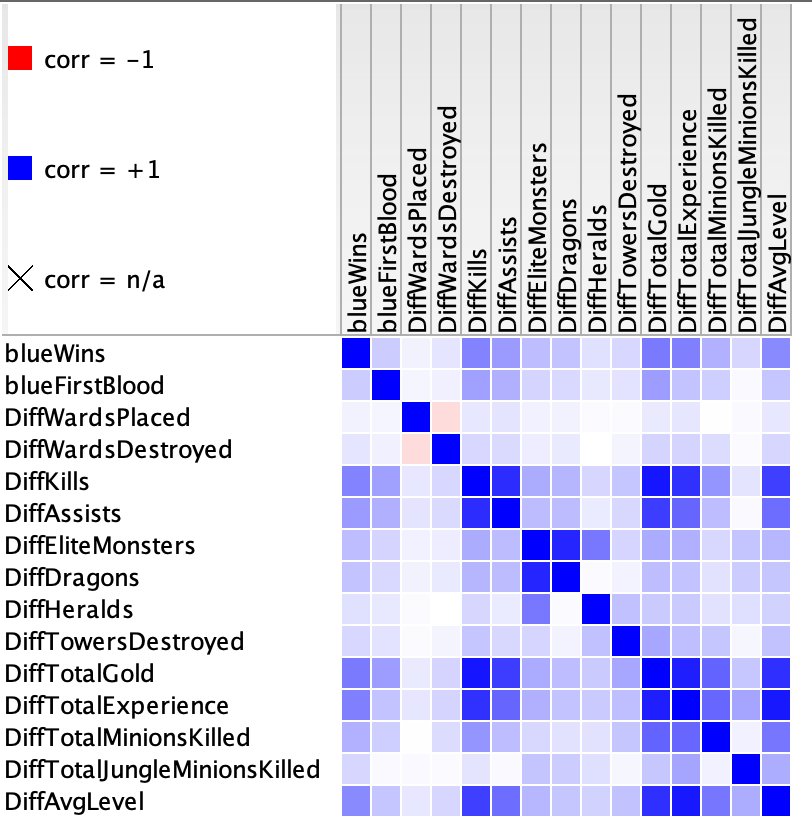
\includegraphics[width=0.5\linewidth]{Figures/RankCorrelation.png}
    \caption{Correlação entre features após processamento.}
    \label{fig:corr1}
\end{figure}

Pela figura \ref{fig:corr1} conseguimos detetar algumas correlações menos óbvios do que obtidas anteriormente. Por exemplo, podemos observar que a diferença em kills está fortemente correlacionada positivamente à diferença em ouro entre as duas equipas.

\begin{figure}[H]
    \centering
    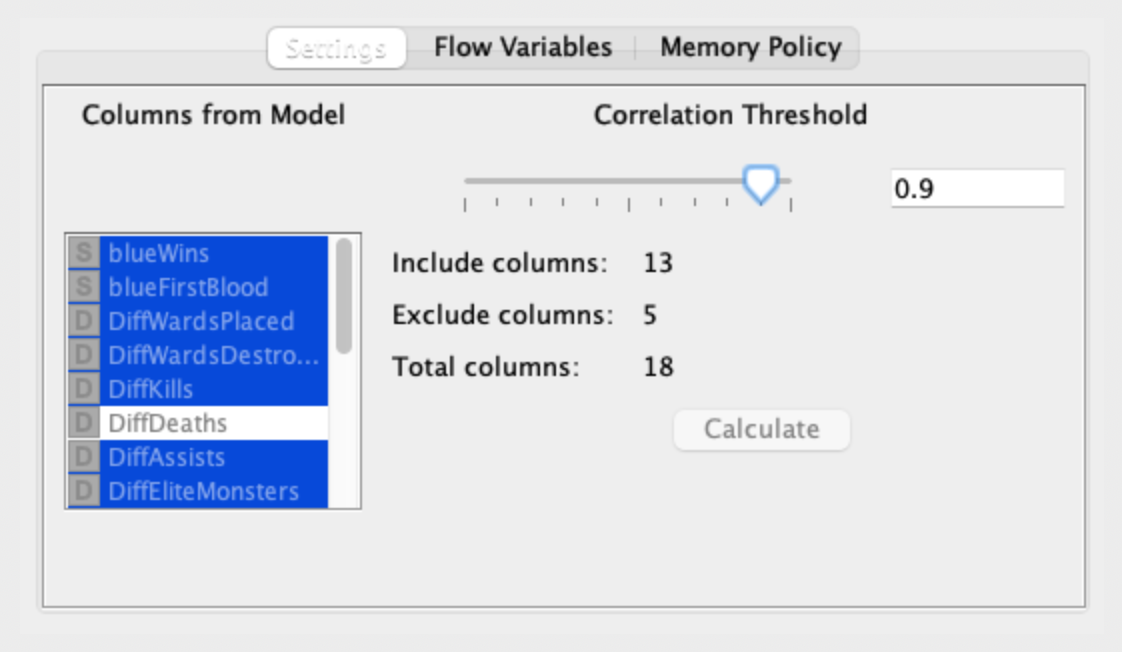
\includegraphics[width=0.5\linewidth]{Figures/Screenshot_2020-11-25_at_22.10.32.png}
    \caption{Seleção automática de features correlacionadas.}
    \label{fig:corr2}
\end{figure}


Como é desnecessário considerar atributos fortemente correlacionados entre si, utilizamos um correlation filter com as configurações da figura \ref{fig:corr2}.

% STEP 4 IN CRISP DM METODOLOGY
\subsection{Modelação}
De forma a garantir a ausência de overfitting decidimos que o ideal seria considerar um modelo baseado em \textit{random forest} que, devido à sua aleatoriadade, permite reduzir fortemente o overfitting.

Com métodos auxiliares de hyper-parameter tuning, fomos capazes de descobrir os hyper-parâmetros ideias para o nosso problema e re-aplicar esses parâmetros directamente na previsão do nosso test set, obtendo uma accuracy perto de 73\%, como se verifica em capítulos adiante. 

% STEP 5 IN CRISP DM METODOLOGY
\subsection{Apreciação dos Modelos}
Utilizando \textit{cross validation} com 10 \textit{folds}, foi possível chegar à conclusão de que a \textit{accuracy} do nosso modelo tende a rondar os 92\% que é, de longe, muito melhores que os nossos modelos iniciais, onde a \textit{accuracy} rondava sempre os 88-89\%. Como tal, este modelo foi seleccionado para ser submetido.

% ---------------------------------------------------------------------------
% 4) LOL (SEM FALAR DE WORKFLOWS)
\section{League of Legends - Liga Diamante}

O \textit{League of Legends} tem vindo a se apresentar como uma nova tendência que atrai cada vez mais jovens, o seu crescimento exponencial levou à criação de uma modalidade de \textit{esports} que desde então tem somado atração pública. Ao longo dos últimos anos, em 2479 torneios, foram atribuídos perto de 80 milhões de dólares em prémios, sendo que o campeonato mundial de 2018 arrecadou um prémio de cerca de 6 milhões de dólares.

Como tal, facilmente conseguimos perceber que o interesse neste tipo de modalidades já não é o simples entretenimento, e que existem quantidade avultadas de dinheiro a ser movidas, o que implica que qualquer análise mais aprofundada aos comportamentos do jogo podem vir a ser lucrativos.

Então, pretendemos tentar modelar os efeitos que os primeiros minutos de jogo podem ter sobre o resultado final de forma a perceber os fatores decisivos numa partida.

% STEP 2 IN CRISP DM METODOLY
\subsection{Compreensão dos Dados}
Para estes dados utilizamos recursos disponíveis na internet\footnote{\url{https://www.kaggle.com/bobbyscience/league-of-legends-diamond-ranked-games-10-min}} e descobrimos um dataset que fornece, de forma sucinta, dados sobre os 10 primeiros minutos das duas equipas (azul e vermelha) utilizando um universo amostral de 10000 membros de uma das ligas mais elevadas do jogo, estes dados incidem exaustivamente sobre todas as metas no jogo como, por exemplo,

\begin{itemize}
    \item Ouro total recolhido, para cada equipa.
    \item Número de execuções, para cada equipa.
    \item Número de wards colocadas, para cada equipa.
\end{itemize}

No total, existem 19 atributos distintos para cada uma das equipa, o que perfaz um total de 38 atributos. Utilizando conhecimento de domínio facilmente conseguimos perceber que ter o mesmo atributo para cada uma das equipas não é indicativo, pelo que seria ideal conseguir agregar ambas as equipas em atributos idênticos.

É também importante denotar que, por conhecimento de domínio, existem atributos que estão necessariamente correlacionados. Por exemplo, o número de execuções da equipa azul e o número de mortes da equipa vermelha estão fortemente correlacionados negativamente, como seria de esperar.

% STEP 3 IN CRISP DM METODOLOGY
\subsection{Preparação dos Dados}
A nível de preparação de dados pouco foi feito, no entanto é importante denotar os seguintes aspectos chaves, que foram cruciais na nossa investigação.

\begin{itemize}
    \item A atributo \texttt{gameID} é completamente irrelevante pois é uma chave única associada a cada jogo, sem nenhum tipo de relevància física, por isso esse atributo foi removido.
    \item Os atributos \texttt{blueWins} e \texttt{redWins} são ambos binários e disjuntos, o que significa que a soma será sempre 1, pois numa dada partida apenas uma equipa pode ganhar. Como tal, consideramos apenas o atributo \texttt{blueWins}, tornando o problema num de prever a vitória ou derrota desta mesma equipa.
    \item De igual forma, os atributos \texttt{blueFirstBlood} e \texttt{redFirstBlood} seguem a mesma condição, pelo que só vale a pena ponderar um destes atributos.
    \item Nos restantes atributos, considerar tanto os atributos da equipa azul e vermelha não faz sentido. Na verdade, estamos interessados em perceber qual a diferença entre os resultados obtidos pela equipa azul num dado atributo e aqueles obtidos pela equipa vermelha. Assim sendo, os restantes atributos, 36, foram reduzidos a 18 por via de \textit{feature engineering}, sendo que no final os atributos em si passam a representar a diferença entre as 2 equipas.
\end{itemize}

Com isto em mente, podemos agora analisar as correlações existentes de forma mais compreensível.

\begin{figure}[H]
    \centering
    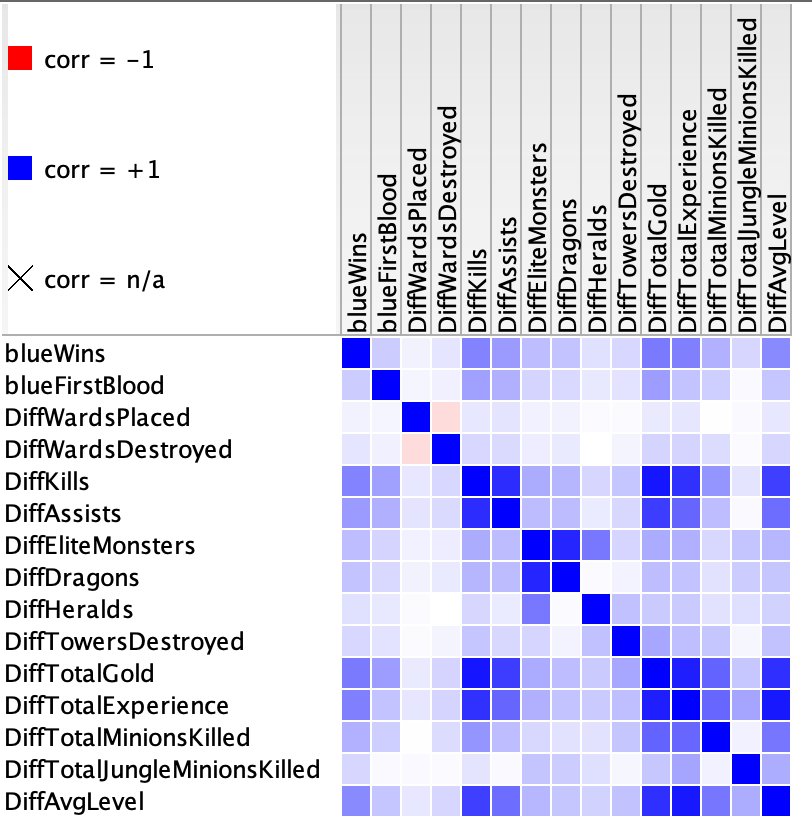
\includegraphics[width=0.5\linewidth]{Figures/RankCorrelation.png}
    \caption{Correlação entre features após processamento.}
    \label{fig:corr1}
\end{figure}

Pela figura \ref{fig:corr1} conseguimos detetar algumas correlações menos óbvios do que obtidas anteriormente. Por exemplo, podemos observar que a diferença em kills está fortemente correlacionada positivamente à diferença em ouro entre as duas equipas.

\begin{figure}[H]
    \centering
    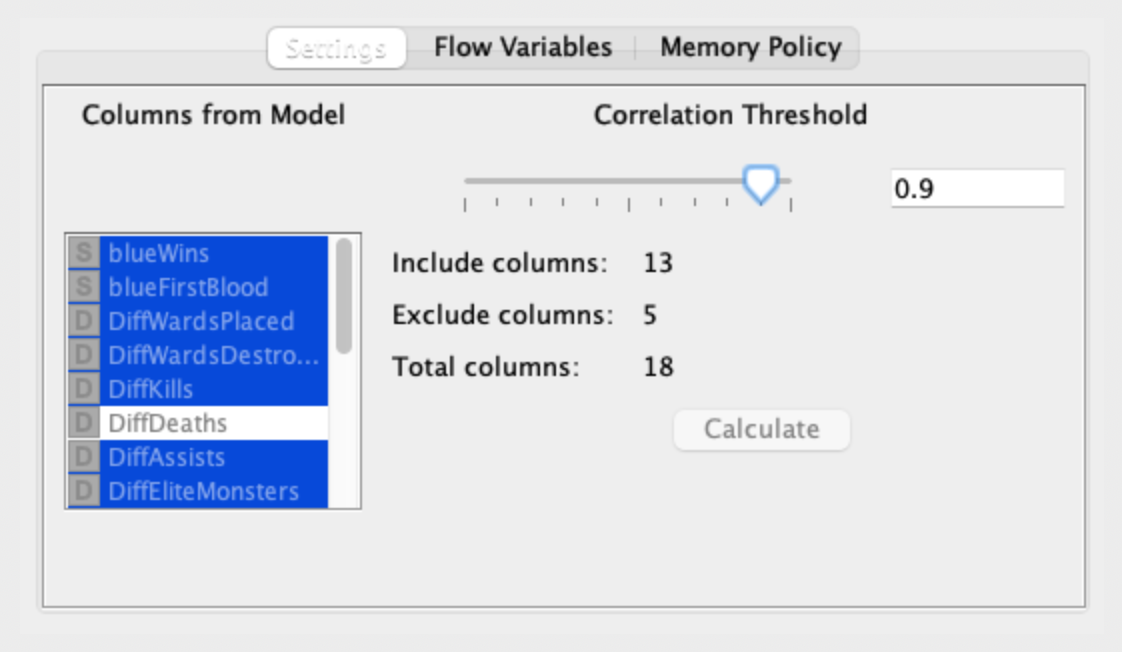
\includegraphics[width=0.5\linewidth]{Figures/Screenshot_2020-11-25_at_22.10.32.png}
    \caption{Seleção automática de features correlacionadas.}
    \label{fig:corr2}
\end{figure}


Como é desnecessário considerar atributos fortemente correlacionados entre si, utilizamos um correlation filter com as configurações da figura \ref{fig:corr2}.

% STEP 4 IN CRISP DM METODOLOGY
\subsection{Modelação}
De forma a garantir a ausência de overfitting decidimos que o ideal seria considerar um modelo baseado em \textit{random forest} que, devido à sua aleatoriadade, permite reduzir fortemente o overfitting.

Com métodos auxiliares de hyper-parameter tuning, fomos capazes de descobrir os hyper-parâmetros ideias para o nosso problema e re-aplicar esses parâmetros directamente na previsão do nosso test set, obtendo uma accuracy perto de 73\%, como se verifica em capítulos adiante. 

% STEP 5 IN CRISP DM METODOLOGY
\subsection{Apreciação dos Modelos}
Utilizando \textit{cross validation} com 10 \textit{folds}, foi possível chegar à conclusão de que a \textit{accuracy} do nosso modelo tende a rondar os 92\% que é, de longe, muito melhores que os nossos modelos iniciais, onde a \textit{accuracy} rondava sempre os 88-89\%. Como tal, este modelo foi seleccionado para ser submetido.

% ---------------------------------------------------------------------------
% 5) KNIME WORKFLOWS
\section{Workflows Desenvolvidos}
\subsection{Acidente em Braga no ano de 2019}
    \subsubsection{Principais nodos}
        \begin{figure}[H]
            \centering
            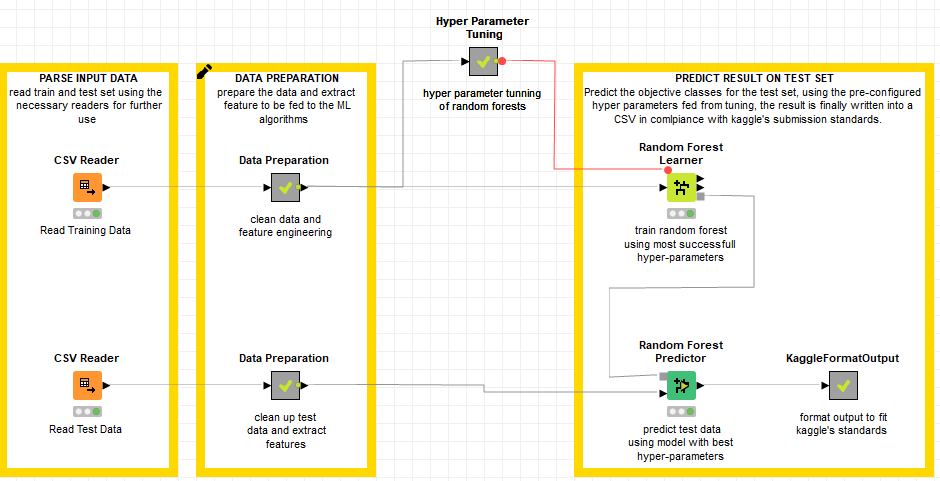
\includegraphics[scale=0.35
            ]{Figures/wf_braga.png}
            \caption{Visão geral do workflow gerado para trabalhar o \textit{dataset}.}
            \label{fig:"um"}
        \end{figure} 
        
    \begin{enumerate}
        \item \textbf{Parse Input Data} \\
            Neste ponto foram carregados para o Knime dois ficheiros, ambos com os mesmos campos de informação, relativos ao número de incidentes rodoviários em Braga. Um dos ficheiros possui dados para usar no treino do modelo, enquanto o outro possui dados para testarmos o modelo.
            
        \item \textbf{Data Preparation} \\
            Relativamente à preparação dos dados apresentamos na figura abaixo o conteúdo do metanodo desenvolvido para esse efeito.
            \begin{figure}[H]
                \centering
                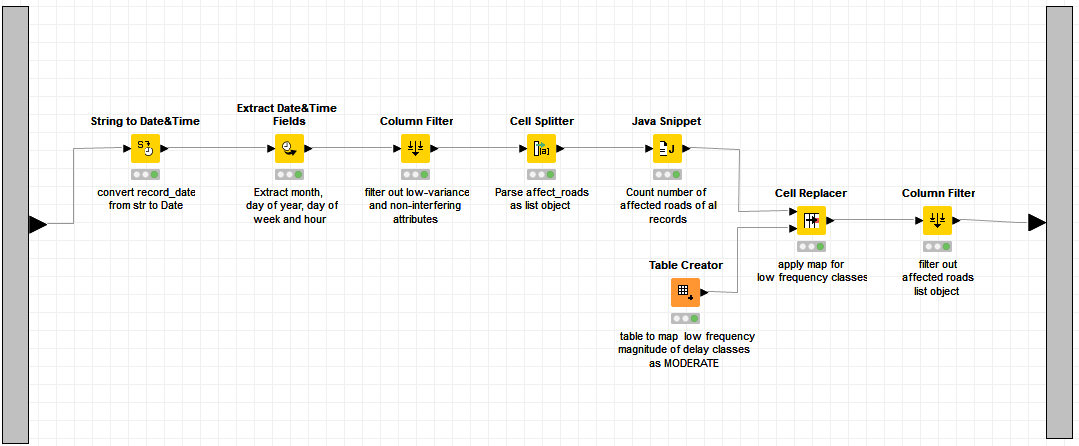
\includegraphics[scale=0.3
                ]{Figures/wf_braga_dataPrep.png}
                \caption{Visão geral do workflow gerado para trabalhar o dataset.}
                \label{fig:"um"}
            \end{figure} 
            De forma geral extraímos, da data inicial, os seguintes valores: mês, dia do ano, dia da semana e hora. De seguida filtramos dados que, através de uma análise de covariância, descobrimos não estarem relacionados ao nível de acidentes. Filtramos também variáveis que possuiam baixa variação, uma vez que também não nos auxiliavam no processo de previsão. Uma vez terminado este ponto extraimos o número de estradas afetas por cada registo. Para tal convertemos a coluna "affect\_roads" de string para lista e, usando a linguagem de programação Java, efetuamos a contagem dos elementos.
            \begin{figure}[H]
                \centering
                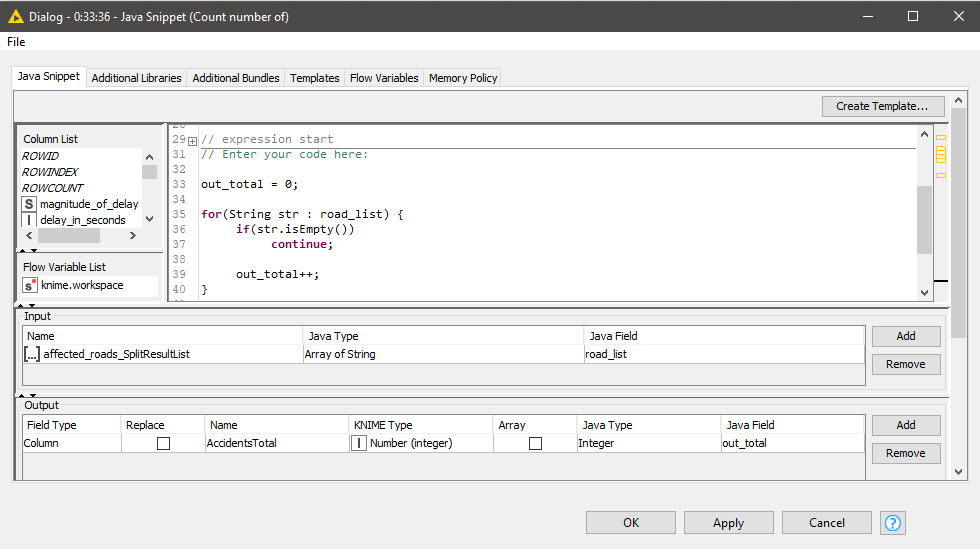
\includegraphics[scale=0.3
                ]{Figures/wf_braga_roadCount.png}
                \caption{Visão geral do workflow gerado para trabalhar o dataset.}
                \label{fig:"um"}
            \end{figure} 
            De seguida convertemos o valor de alguns campos relativos a "magnitude\_of\_delay". Optámos por converter as classes deste campo que tinham uma baixa frequência para a classe "MODERATE".
            
        \item \textbf{Hyper Parameter Tuning} \\
            Para melhorarmos a precisão do modelo gerado optamos por fazer um "tuning" dos parâmetros utilizados. Para o fazer utilizamos loops, testando diferentes combinações entre os critérios de divisão de Random Forests e múltiplos valores para o número de modelos e profundidade da árvore. Uma vez terminados estes loops passamos os valores obtidos como "ideais" para variável de flow e treinamos um modelo com estas definições, já no próximo ponto. Pode ser vista uma representação desta parte do processo mais á frente, mais concretamente na secção "Descrição do modelo gerado".
        
        \item \textbf{Previsões} \\
            Uma vez optimizados os parâmetros do modelo procedemos ao treino do mesmo, para o efeito utilizando um \textit{Random Forest Learner}. Com o modelo gerado prevemos o nível de acidentes para cada um dos registos presentes no \textit{dataset} de teste. Os resultados desta previsão são então exportados, de acordo com as regras estabelecidas para a competição na plataforma \textit{Kaggle}.
    \end{enumerate}
    
    \subsubsection{Descrição do modelo gerado}
        \begin{enumerate}
            \item \textbf{Tuning}    
                \begin{figure}[H]
                    \centering
                    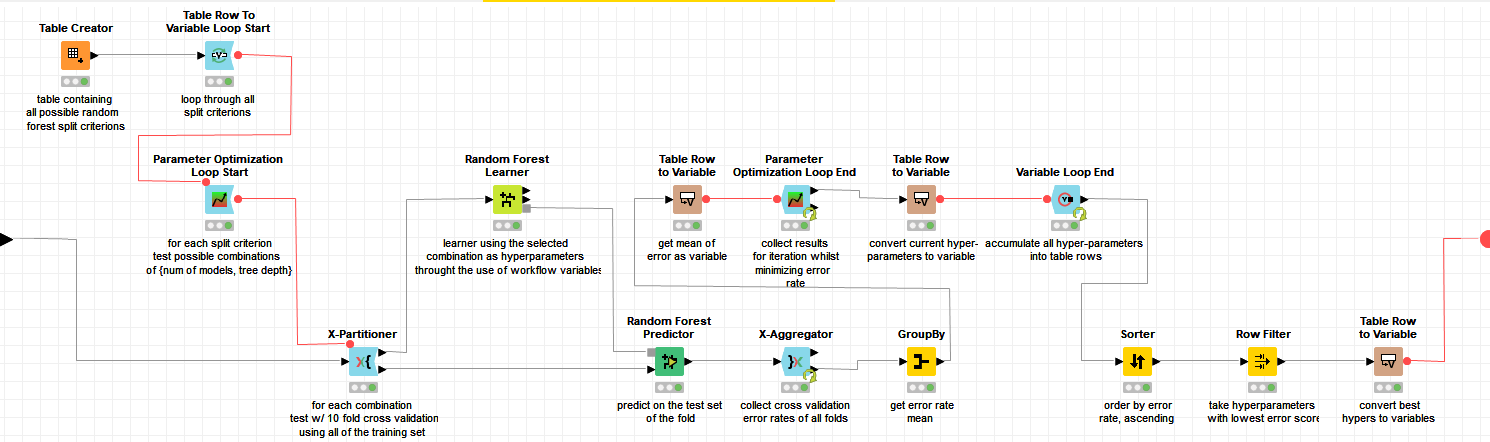
\includegraphics[scale=0.30
                    ]{Figures/wf_braga_hyper.png}
                    \caption{Metanodo utilizado para optimização do hiper-parâmetros.}
                    \label{fig:"um"}
                \end{figure} 
                
            \item \textbf{Características do treino}
                Após terminado o loop de optimização temos então os valores óptimos para a nossa \textit{Decision Tree}. No caso em concreto os parametros "ideais" foram os seguintes:
                \begin{itemize}
                    \item Número de modelos: 700
                    \item Profundidade da árvore: 25
                    \item Split Criterions: Information Gain
                \end{itemize}
                \begin{figure}[H]
                    \centering
                    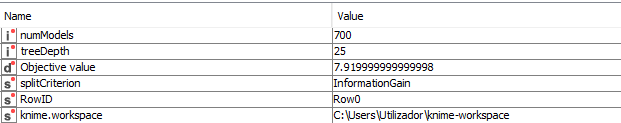
\includegraphics[scale=0.30
                    ]{Figures/wf_braga_hyperdata.png}
                    \caption{Settings utilizados para treino do modelo.}
                    \label{fig:"um"}
                \end{figure} 
        \end{enumerate}

\subsection{League of Legends - previsão baseada nos 10 primeiros minutos de jogo}
    \subsubsection{Principais nodos}
        \begin{figure}[H]
            \centering
            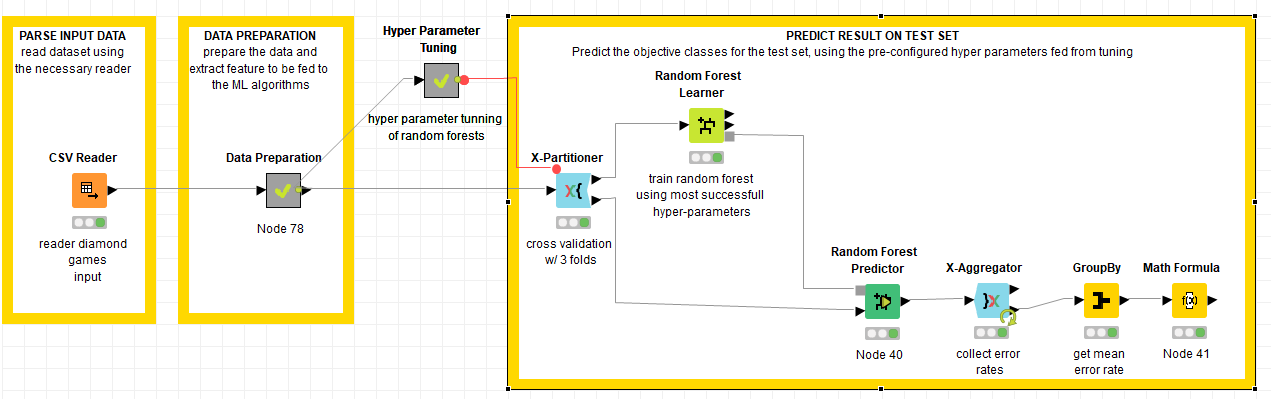
\includegraphics[scale=0.30
            ]{Figures/wf_lol.png}
            \caption{Visão geral do workflow gerado para trabalhar o dataset.}
            \label{fig:"um"}
        \end{figure} 
        
    \begin{enumerate}
        \item \textbf{Parse Input Data} \\
            Como ponto inicial do nosso processo tivemos que ler os dados a serem utilizados. Os dados originais encontravam-se num ficheiro .csv, assim sendo utilizamos o nodo CSV Reader.
        
        \item \textbf{Data Preparation} \\
            Após carregados os dados, passamos ao tratamento/preparação dos mesmos. Para tal desenvolvemos o workflow presente na figura abaixo.
            \begin{figure}[H]
                \centering
                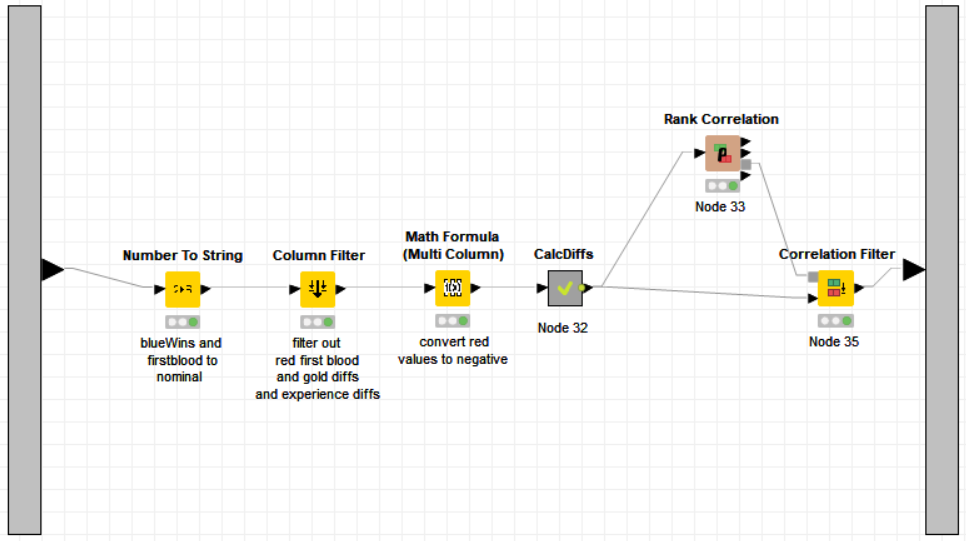
\includegraphics[scale=0.30
                ]{Figures/wf_lol_data.png}
                \caption{Visão geral do workflow gerado para trabalhar o dataset.}
                \label{fig:"um"}
            \end{figure} 
            Os dados presentes em cada registo, como já referido antes, eram bastante redundantes, uma vez que o \textit{dataset} possuía todos os dados para ambas as equipas. Desta forma optámos por transformar estes dados num diferencial. Como exemplo, no \textit{dataset}, antes do tratamento, tínhamos dados como o número de mortes que a equipa azul causou e o número de mortes que a equipa vermelha causou. Depois deste processo deixamos de ter estas duas colunas e passamos a ter uma variável que indica a diferença entre o número de mortes causadas por cada equipa. Por fim aplicamos um \textit{correlation filter}, com um \textit{treshold} de quase 1, de forma a eliminar automaticamente as colunas que podiam praticamente ser obtidas a partir das restantes, como por exemplo a diferença entre o número de jogadores mortos pelas equipas e a diferença de vezes que cada equipa morreu.
        
        \item \textbf{Hyper Parameter Tuning} \\
            Para fazermos o tuning utilizamos o metanodo que previamente desenvolvemos para treinar o modelo para a competição de \textit{Kaggle}. Desta forma o funcionamento do mesmo não será explicitado neste ponto, uma vez que seria repetitivo.
        \item \textbf{Previsões} \\
            A partir do momento que temos os parâmetros óptimos para o nosso modelo podemos finalmente treinar e testar o mesmo. Para tal utilizamos o nodo "X Partitioner", utilizando 3 folds. Uma vez terminado este processo calculamos a precisão do modelo, considerando que o método de agrupamento dos resultados nos retorna a média do erro entre as 3 folds.
    \end{enumerate}
        
    \subsubsection{Descrição do modelo gerado}
        \begin{enumerate}
            \item \textbf{Tuning}\\
                Pelo motivo referido acima, não iremos entrar em detalhe neste ponto. Existe uma descrição detalhada do mesmo nos pontos 4.1.1 e 4.1.2
            \item \textbf{Características do treino}\\
                Após terminado o loop de optimização temos então os valores óptimos para a nossa \textit{Decision Tree}. No caso em concreto os parâmetros "ideais" foram os seguintes:
                \begin{itemize}
                    \item Número de modelos: 500
                    \item Profundidade da árvore: 10
                    \item Split Criterions: Information Gain
                \end{itemize}
                \begin{figure}[H]
                    \centering
                    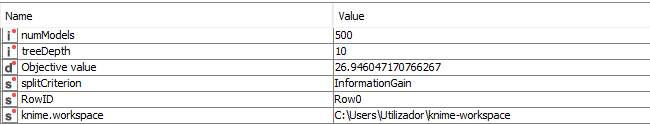
\includegraphics[scale=0.30
                    ]{Figures/wf_lol_hyperdata.png}
                    \caption{Settings utilizados para treino do modelo.}
                    \label{fig:"um"}
                \end{figure} 
        \end{enumerate}


% ---------------------------------------------------------------------------
% 6) SUGESTOES E RECOMENDACOES
\section{Sugestões \& Recomendações}

\subsection{Acidentes em Braga no ano de 2019}

Ao longo do desenvolvimento do nosso projeto percebemos, analisando os resultados finais, que existe uma diferença muito pouco definida entre o conjunto de classes $\{\mbox{\texttt{Low}, \texttt{Medium}, \texttt{High}}\}$ pelo que o nosso modelo, segundo as curvas ROC, é péssimo a distinguir entre estas classes. Apesar de ser muito bom a distinguir entre as classes $\{\mbox{\texttt{None}, \texttt{Very High}}\}$, uma performance na melhoria da accuracy está diretamente relacionada com a boa separação classes, o que não é de todo garantido com o modelo atual. 

\begin{figure}[H]
    \centering
    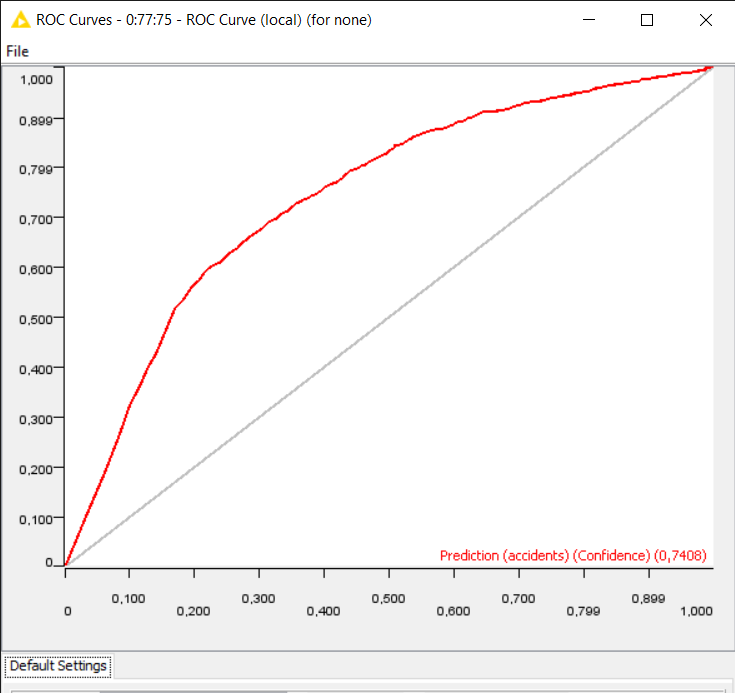
\includegraphics[width=0.4\linewidth]{Figures/ROC/none.png}
    \caption{Curva de ROC para a classe \texttt{None}.}
    \label{fig:ii1}
\end{figure}

\begin{figure}[H]
    \centering
    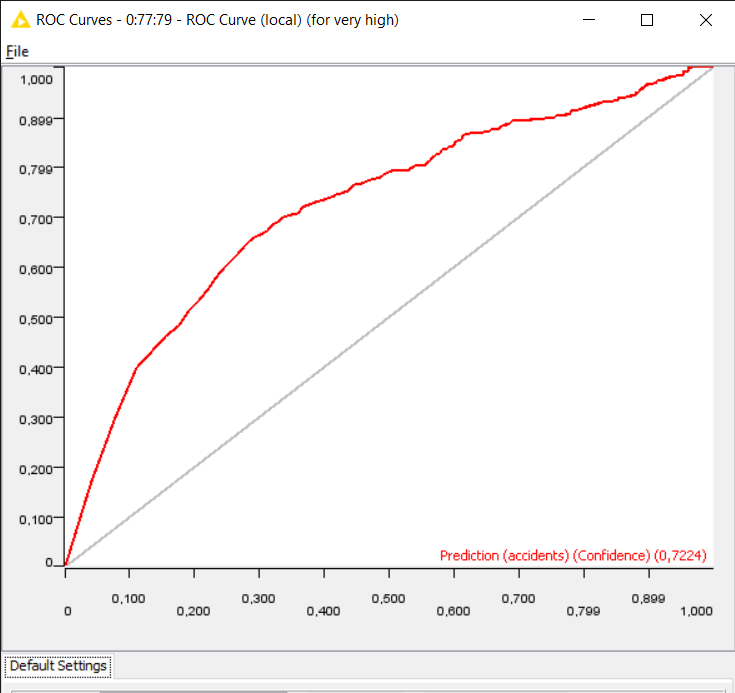
\includegraphics[width=0.4\linewidth]{Figures/ROC/very high.png}
    \caption{Curva de ROC para a classe \texttt{Very High}.}
    \label{fig:ii2}
\end{figure}

Como podemos ver pelas figuras \ref{fig:ii1} e \ref{fig:ii2} rapidamente percebemos que o nosso modelo consegue fazer uma boa distinção entre estas duas. No entanto, se olharmos para as figuras \ref{fig:ii3}, \ref{fig:ii4} e \ref{fig:ii5}, rapidamente percebemos que o nosso modelo é péssimo nestas classes.

\begin{figure}[H]
    \centering
    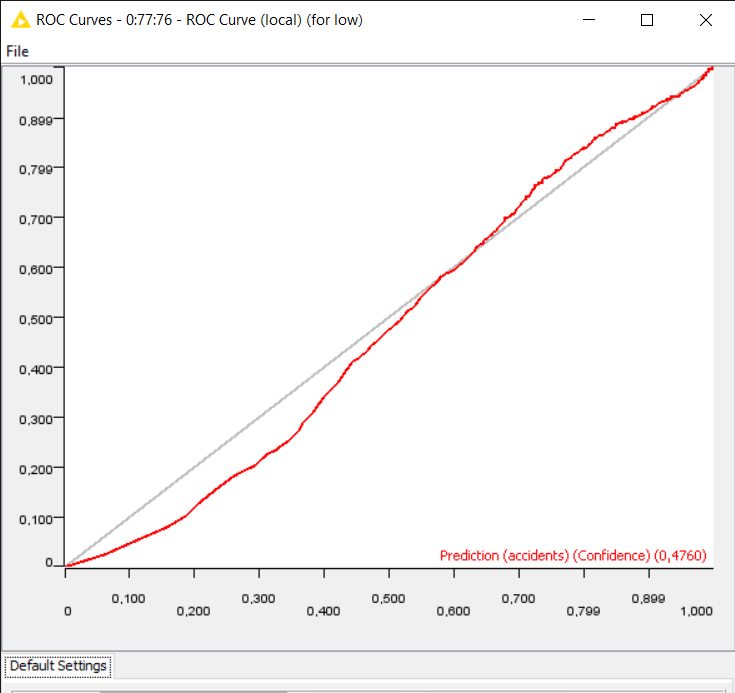
\includegraphics[width=0.4\linewidth]{Figures/ROC/low.png}
    \caption{Curva de ROC para a classe \texttt{Low}.}
    \label{fig:ii3}
\end{figure}

\begin{figure}[H]
    \centering
    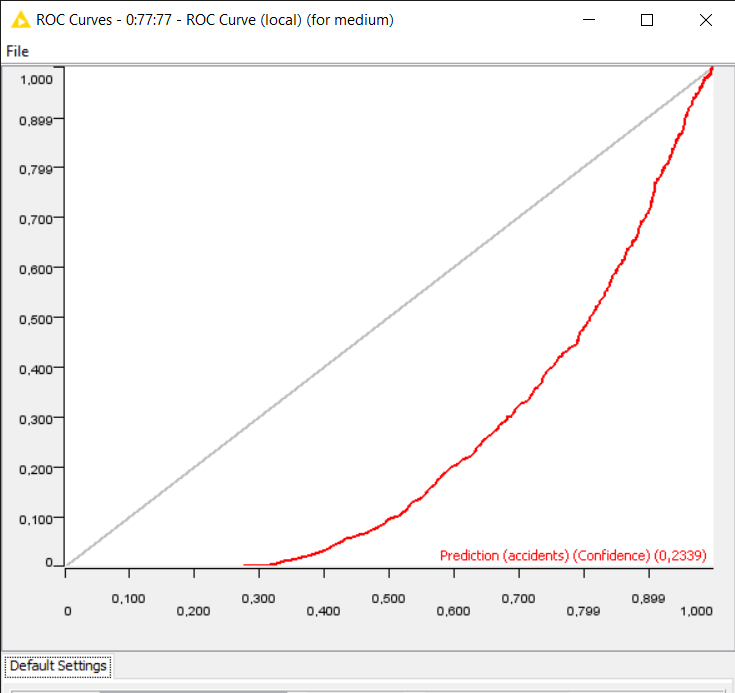
\includegraphics[width=0.4\linewidth]{Figures/ROC/medium.png}
    \caption{Curva de ROC para a classe \texttt{Medium}.}
    \label{fig:ii4}
\end{figure}

\begin{figure}[H]
    \centering
    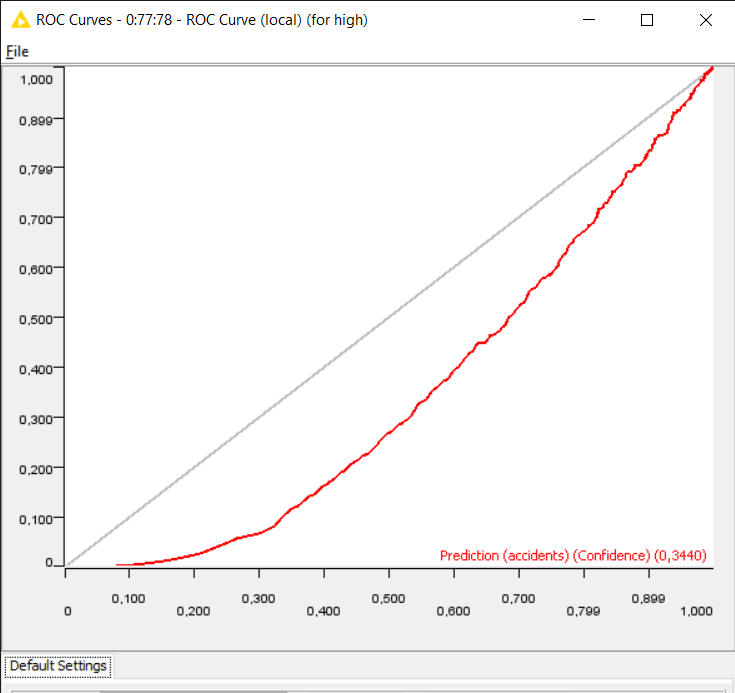
\includegraphics[width=0.4\linewidth]{Figures/ROC/high.png}
    \caption{Curva de ROC para a classe \texttt{High}.}
    \label{fig:ii5}
\end{figure}

\subsection{League of Legends}

Apesar dos resultados bastante promissores apenas com os primeiros 10 minutos de jogo, é notável que, num jogo com dinâmicas tão complexas, utilizar apenas os primeiros 10 minutos é pouco representativo no resultado final.

Existem muitos objetivos, como batalhas em equipa e obtenção de monstros épicos que fornecem pontos de viragem cruciais em jogos, que tendem a concentrarem-se em períodos após os primeiros 10 minutos.

Como tal, e em formato de recomendação, ponderamos que com um aumento do número de minutos considerados poderemos vir a obter \textit{accuracies} mais elavadas. 

% ---------------------------------------------------------------------------
% 7) CONCLUSÃO
\section{Conclusão}
Uma vez terminada a exposição do trabalho efectuado podemos então tirar algumas conclusões sobre o mesmo. 

Como ponto inicial começamos por ressalvar a utilidade da metodologia CRISP-DM ao longo deste projeto. Serviu não só para garantir a qualidade dos modelos desenvolvidos como também para estruturar e organizar o desenvolvimento do projeto. Consideramos que esta metodologia foi, em parte, responsável pelos bons resultados obtidos, quer na exploração do \textit{dataset} relativo a acidentes em Braga em 2019, quer na exploração do \textit{dataset} relativo ao videojogo League of Legends. 

Incidindo então concretamente sobre os modelos gerados, de uma forma geral estamos satisfeitos com os resultados obtidos. Conseguimos uma precisão alta com o modelo gerado para prever a magnitude de incidentes rodoviários na cidade de Braga, obtendo uma precisão final de cerca de 92\% de acertos, reflexo também da exploração e preparação dos dados por nós feita.

Relativamente ao modelo desenhado para prever o vencedor de partidas de League of Legends, embora à primeira vista a precisão possa parecer baixa, rondando os 73\%, consideramos que foi também este um resultado bastante bom, confirmando que realmente existe um impacto grande dos 10 primeiros minutos de jogo no resultado final da partida.

Assim sendo, considerando os processos desenvolvidos, apresentados neste relatório,  e os resultados dos mesmo, consideramos que conseguimos obter resultados satisfatórios em ambos os modelos desenvolvidos. Conseguimos ainda identificar pontos que poderiam ser trabalhados/modificados de forma a conseguir resultados ainda melhores. 


\newpage
\printnoidxglossaries
\end{document}